
% Default to the notebook output style

    


% Inherit from the specified cell style.




    
\documentclass[11pt]{article}

    
    
    \usepackage[T1]{fontenc}
    % Nicer default font (+ math font) than Computer Modern for most use cases
    \usepackage{mathpazo}

    % Basic figure setup, for now with no caption control since it's done
    % automatically by Pandoc (which extracts ![](path) syntax from Markdown).
    \usepackage{graphicx}
    % We will generate all images so they have a width \maxwidth. This means
    % that they will get their normal width if they fit onto the page, but
    % are scaled down if they would overflow the margins.
    \makeatletter
    \def\maxwidth{\ifdim\Gin@nat@width>\linewidth\linewidth
    \else\Gin@nat@width\fi}
    \makeatother
    \let\Oldincludegraphics\includegraphics
    % Set max figure width to be 80% of text width, for now hardcoded.
    \renewcommand{\includegraphics}[1]{\Oldincludegraphics[width=.8\maxwidth]{#1}}
    % Ensure that by default, figures have no caption (until we provide a
    % proper Figure object with a Caption API and a way to capture that
    % in the conversion process - todo).
    \usepackage{caption}
    \DeclareCaptionLabelFormat{nolabel}{}
    \captionsetup{labelformat=nolabel}

    \usepackage{adjustbox} % Used to constrain images to a maximum size 
    \usepackage{xcolor} % Allow colors to be defined
    \usepackage{enumerate} % Needed for markdown enumerations to work
    \usepackage{geometry} % Used to adjust the document margins
    \usepackage{amsmath} % Equations
    \usepackage{amssymb} % Equations
    \usepackage{textcomp} % defines textquotesingle
    % Hack from http://tex.stackexchange.com/a/47451/13684:
    \AtBeginDocument{%
        \def\PYZsq{\textquotesingle}% Upright quotes in Pygmentized code
    }
    \usepackage{upquote} % Upright quotes for verbatim code
    \usepackage{eurosym} % defines \euro
    \usepackage[mathletters]{ucs} % Extended unicode (utf-8) support
    \usepackage[utf8x]{inputenc} % Allow utf-8 characters in the tex document
    \usepackage{fancyvrb} % verbatim replacement that allows latex
    \usepackage{grffile} % extends the file name processing of package graphics 
                         % to support a larger range 
    % The hyperref package gives us a pdf with properly built
    % internal navigation ('pdf bookmarks' for the table of contents,
    % internal cross-reference links, web links for URLs, etc.)
    \usepackage{hyperref}
    \usepackage{longtable} % longtable support required by pandoc >1.10
    \usepackage{booktabs}  % table support for pandoc > 1.12.2
    \usepackage[inline]{enumitem} % IRkernel/repr support (it uses the enumerate* environment)
    \usepackage[normalem]{ulem} % ulem is needed to support strikethroughs (\sout)
                                % normalem makes italics be italics, not underlines
    
    
    % Colors for the hyperref package
    \definecolor{urlcolor}{rgb}{0,.145,.698}
    \definecolor{linkcolor}{rgb}{.71,0.21,0.01}
    \definecolor{citecolor}{rgb}{.12,.54,.11}

    % ANSI colors
    \definecolor{ansi-black}{HTML}{3E424D}
    \definecolor{ansi-black-intense}{HTML}{282C36}
    \definecolor{ansi-red}{HTML}{E75C58}
    \definecolor{ansi-red-intense}{HTML}{B22B31}
    \definecolor{ansi-green}{HTML}{00A250}
    \definecolor{ansi-green-intense}{HTML}{007427}
    \definecolor{ansi-yellow}{HTML}{DDB62B}
    \definecolor{ansi-yellow-intense}{HTML}{B27D12}
    \definecolor{ansi-blue}{HTML}{208FFB}
    \definecolor{ansi-blue-intense}{HTML}{0065CA}
    \definecolor{ansi-magenta}{HTML}{D160C4}
    \definecolor{ansi-magenta-intense}{HTML}{A03196}
    \definecolor{ansi-cyan}{HTML}{60C6C8}
    \definecolor{ansi-cyan-intense}{HTML}{258F8F}
    \definecolor{ansi-white}{HTML}{C5C1B4}
    \definecolor{ansi-white-intense}{HTML}{A1A6B2}

    % commands and environments needed by pandoc snippets
    % extracted from the output of `pandoc -s`
    \providecommand{\tightlist}{%
      \setlength{\itemsep}{0pt}\setlength{\parskip}{0pt}}
    \DefineVerbatimEnvironment{Highlighting}{Verbatim}{commandchars=\\\{\}}
    % Add ',fontsize=\small' for more characters per line
    \newenvironment{Shaded}{}{}
    \newcommand{\KeywordTok}[1]{\textcolor[rgb]{0.00,0.44,0.13}{\textbf{{#1}}}}
    \newcommand{\DataTypeTok}[1]{\textcolor[rgb]{0.56,0.13,0.00}{{#1}}}
    \newcommand{\DecValTok}[1]{\textcolor[rgb]{0.25,0.63,0.44}{{#1}}}
    \newcommand{\BaseNTok}[1]{\textcolor[rgb]{0.25,0.63,0.44}{{#1}}}
    \newcommand{\FloatTok}[1]{\textcolor[rgb]{0.25,0.63,0.44}{{#1}}}
    \newcommand{\CharTok}[1]{\textcolor[rgb]{0.25,0.44,0.63}{{#1}}}
    \newcommand{\StringTok}[1]{\textcolor[rgb]{0.25,0.44,0.63}{{#1}}}
    \newcommand{\CommentTok}[1]{\textcolor[rgb]{0.38,0.63,0.69}{\textit{{#1}}}}
    \newcommand{\OtherTok}[1]{\textcolor[rgb]{0.00,0.44,0.13}{{#1}}}
    \newcommand{\AlertTok}[1]{\textcolor[rgb]{1.00,0.00,0.00}{\textbf{{#1}}}}
    \newcommand{\FunctionTok}[1]{\textcolor[rgb]{0.02,0.16,0.49}{{#1}}}
    \newcommand{\RegionMarkerTok}[1]{{#1}}
    \newcommand{\ErrorTok}[1]{\textcolor[rgb]{1.00,0.00,0.00}{\textbf{{#1}}}}
    \newcommand{\NormalTok}[1]{{#1}}
    
    % Additional commands for more recent versions of Pandoc
    \newcommand{\ConstantTok}[1]{\textcolor[rgb]{0.53,0.00,0.00}{{#1}}}
    \newcommand{\SpecialCharTok}[1]{\textcolor[rgb]{0.25,0.44,0.63}{{#1}}}
    \newcommand{\VerbatimStringTok}[1]{\textcolor[rgb]{0.25,0.44,0.63}{{#1}}}
    \newcommand{\SpecialStringTok}[1]{\textcolor[rgb]{0.73,0.40,0.53}{{#1}}}
    \newcommand{\ImportTok}[1]{{#1}}
    \newcommand{\DocumentationTok}[1]{\textcolor[rgb]{0.73,0.13,0.13}{\textit{{#1}}}}
    \newcommand{\AnnotationTok}[1]{\textcolor[rgb]{0.38,0.63,0.69}{\textbf{\textit{{#1}}}}}
    \newcommand{\CommentVarTok}[1]{\textcolor[rgb]{0.38,0.63,0.69}{\textbf{\textit{{#1}}}}}
    \newcommand{\VariableTok}[1]{\textcolor[rgb]{0.10,0.09,0.49}{{#1}}}
    \newcommand{\ControlFlowTok}[1]{\textcolor[rgb]{0.00,0.44,0.13}{\textbf{{#1}}}}
    \newcommand{\OperatorTok}[1]{\textcolor[rgb]{0.40,0.40,0.40}{{#1}}}
    \newcommand{\BuiltInTok}[1]{{#1}}
    \newcommand{\ExtensionTok}[1]{{#1}}
    \newcommand{\PreprocessorTok}[1]{\textcolor[rgb]{0.74,0.48,0.00}{{#1}}}
    \newcommand{\AttributeTok}[1]{\textcolor[rgb]{0.49,0.56,0.16}{{#1}}}
    \newcommand{\InformationTok}[1]{\textcolor[rgb]{0.38,0.63,0.69}{\textbf{\textit{{#1}}}}}
    \newcommand{\WarningTok}[1]{\textcolor[rgb]{0.38,0.63,0.69}{\textbf{\textit{{#1}}}}}
    
    
    % Define a nice break command that doesn't care if a line doesn't already
    % exist.
    \def\br{\hspace*{\fill} \\* }
    % Math Jax compatability definitions
    \def\gt{>}
    \def\lt{<}
    % Document parameters
    \title{4.5 Lokale Operatoren/Sobel-Operator}
        

    % Pygments definitions
    
\makeatletter
\def\PY@reset{\let\PY@it=\relax \let\PY@bf=\relax%
    \let\PY@ul=\relax \let\PY@tc=\relax%
    \let\PY@bc=\relax \let\PY@ff=\relax}
\def\PY@tok#1{\csname PY@tok@#1\endcsname}
\def\PY@toks#1+{\ifx\relax#1\empty\else%
    \PY@tok{#1}\expandafter\PY@toks\fi}
\def\PY@do#1{\PY@bc{\PY@tc{\PY@ul{%
    \PY@it{\PY@bf{\PY@ff{#1}}}}}}}
\def\PY#1#2{\PY@reset\PY@toks#1+\relax+\PY@do{#2}}

\expandafter\def\csname PY@tok@gd\endcsname{\def\PY@tc##1{\textcolor[rgb]{0.63,0.00,0.00}{##1}}}
\expandafter\def\csname PY@tok@gu\endcsname{\let\PY@bf=\textbf\def\PY@tc##1{\textcolor[rgb]{0.50,0.00,0.50}{##1}}}
\expandafter\def\csname PY@tok@gt\endcsname{\def\PY@tc##1{\textcolor[rgb]{0.00,0.27,0.87}{##1}}}
\expandafter\def\csname PY@tok@gs\endcsname{\let\PY@bf=\textbf}
\expandafter\def\csname PY@tok@gr\endcsname{\def\PY@tc##1{\textcolor[rgb]{1.00,0.00,0.00}{##1}}}
\expandafter\def\csname PY@tok@cm\endcsname{\let\PY@it=\textit\def\PY@tc##1{\textcolor[rgb]{0.25,0.50,0.50}{##1}}}
\expandafter\def\csname PY@tok@vg\endcsname{\def\PY@tc##1{\textcolor[rgb]{0.10,0.09,0.49}{##1}}}
\expandafter\def\csname PY@tok@vi\endcsname{\def\PY@tc##1{\textcolor[rgb]{0.10,0.09,0.49}{##1}}}
\expandafter\def\csname PY@tok@vm\endcsname{\def\PY@tc##1{\textcolor[rgb]{0.10,0.09,0.49}{##1}}}
\expandafter\def\csname PY@tok@mh\endcsname{\def\PY@tc##1{\textcolor[rgb]{0.40,0.40,0.40}{##1}}}
\expandafter\def\csname PY@tok@cs\endcsname{\let\PY@it=\textit\def\PY@tc##1{\textcolor[rgb]{0.25,0.50,0.50}{##1}}}
\expandafter\def\csname PY@tok@ge\endcsname{\let\PY@it=\textit}
\expandafter\def\csname PY@tok@vc\endcsname{\def\PY@tc##1{\textcolor[rgb]{0.10,0.09,0.49}{##1}}}
\expandafter\def\csname PY@tok@il\endcsname{\def\PY@tc##1{\textcolor[rgb]{0.40,0.40,0.40}{##1}}}
\expandafter\def\csname PY@tok@go\endcsname{\def\PY@tc##1{\textcolor[rgb]{0.53,0.53,0.53}{##1}}}
\expandafter\def\csname PY@tok@cp\endcsname{\def\PY@tc##1{\textcolor[rgb]{0.74,0.48,0.00}{##1}}}
\expandafter\def\csname PY@tok@gi\endcsname{\def\PY@tc##1{\textcolor[rgb]{0.00,0.63,0.00}{##1}}}
\expandafter\def\csname PY@tok@gh\endcsname{\let\PY@bf=\textbf\def\PY@tc##1{\textcolor[rgb]{0.00,0.00,0.50}{##1}}}
\expandafter\def\csname PY@tok@ni\endcsname{\let\PY@bf=\textbf\def\PY@tc##1{\textcolor[rgb]{0.60,0.60,0.60}{##1}}}
\expandafter\def\csname PY@tok@nl\endcsname{\def\PY@tc##1{\textcolor[rgb]{0.63,0.63,0.00}{##1}}}
\expandafter\def\csname PY@tok@nn\endcsname{\let\PY@bf=\textbf\def\PY@tc##1{\textcolor[rgb]{0.00,0.00,1.00}{##1}}}
\expandafter\def\csname PY@tok@no\endcsname{\def\PY@tc##1{\textcolor[rgb]{0.53,0.00,0.00}{##1}}}
\expandafter\def\csname PY@tok@na\endcsname{\def\PY@tc##1{\textcolor[rgb]{0.49,0.56,0.16}{##1}}}
\expandafter\def\csname PY@tok@nb\endcsname{\def\PY@tc##1{\textcolor[rgb]{0.00,0.50,0.00}{##1}}}
\expandafter\def\csname PY@tok@nc\endcsname{\let\PY@bf=\textbf\def\PY@tc##1{\textcolor[rgb]{0.00,0.00,1.00}{##1}}}
\expandafter\def\csname PY@tok@nd\endcsname{\def\PY@tc##1{\textcolor[rgb]{0.67,0.13,1.00}{##1}}}
\expandafter\def\csname PY@tok@ne\endcsname{\let\PY@bf=\textbf\def\PY@tc##1{\textcolor[rgb]{0.82,0.25,0.23}{##1}}}
\expandafter\def\csname PY@tok@nf\endcsname{\def\PY@tc##1{\textcolor[rgb]{0.00,0.00,1.00}{##1}}}
\expandafter\def\csname PY@tok@si\endcsname{\let\PY@bf=\textbf\def\PY@tc##1{\textcolor[rgb]{0.73,0.40,0.53}{##1}}}
\expandafter\def\csname PY@tok@s2\endcsname{\def\PY@tc##1{\textcolor[rgb]{0.73,0.13,0.13}{##1}}}
\expandafter\def\csname PY@tok@nt\endcsname{\let\PY@bf=\textbf\def\PY@tc##1{\textcolor[rgb]{0.00,0.50,0.00}{##1}}}
\expandafter\def\csname PY@tok@nv\endcsname{\def\PY@tc##1{\textcolor[rgb]{0.10,0.09,0.49}{##1}}}
\expandafter\def\csname PY@tok@s1\endcsname{\def\PY@tc##1{\textcolor[rgb]{0.73,0.13,0.13}{##1}}}
\expandafter\def\csname PY@tok@dl\endcsname{\def\PY@tc##1{\textcolor[rgb]{0.73,0.13,0.13}{##1}}}
\expandafter\def\csname PY@tok@ch\endcsname{\let\PY@it=\textit\def\PY@tc##1{\textcolor[rgb]{0.25,0.50,0.50}{##1}}}
\expandafter\def\csname PY@tok@m\endcsname{\def\PY@tc##1{\textcolor[rgb]{0.40,0.40,0.40}{##1}}}
\expandafter\def\csname PY@tok@gp\endcsname{\let\PY@bf=\textbf\def\PY@tc##1{\textcolor[rgb]{0.00,0.00,0.50}{##1}}}
\expandafter\def\csname PY@tok@sh\endcsname{\def\PY@tc##1{\textcolor[rgb]{0.73,0.13,0.13}{##1}}}
\expandafter\def\csname PY@tok@ow\endcsname{\let\PY@bf=\textbf\def\PY@tc##1{\textcolor[rgb]{0.67,0.13,1.00}{##1}}}
\expandafter\def\csname PY@tok@sx\endcsname{\def\PY@tc##1{\textcolor[rgb]{0.00,0.50,0.00}{##1}}}
\expandafter\def\csname PY@tok@bp\endcsname{\def\PY@tc##1{\textcolor[rgb]{0.00,0.50,0.00}{##1}}}
\expandafter\def\csname PY@tok@c1\endcsname{\let\PY@it=\textit\def\PY@tc##1{\textcolor[rgb]{0.25,0.50,0.50}{##1}}}
\expandafter\def\csname PY@tok@fm\endcsname{\def\PY@tc##1{\textcolor[rgb]{0.00,0.00,1.00}{##1}}}
\expandafter\def\csname PY@tok@o\endcsname{\def\PY@tc##1{\textcolor[rgb]{0.40,0.40,0.40}{##1}}}
\expandafter\def\csname PY@tok@kc\endcsname{\let\PY@bf=\textbf\def\PY@tc##1{\textcolor[rgb]{0.00,0.50,0.00}{##1}}}
\expandafter\def\csname PY@tok@c\endcsname{\let\PY@it=\textit\def\PY@tc##1{\textcolor[rgb]{0.25,0.50,0.50}{##1}}}
\expandafter\def\csname PY@tok@mf\endcsname{\def\PY@tc##1{\textcolor[rgb]{0.40,0.40,0.40}{##1}}}
\expandafter\def\csname PY@tok@err\endcsname{\def\PY@bc##1{\setlength{\fboxsep}{0pt}\fcolorbox[rgb]{1.00,0.00,0.00}{1,1,1}{\strut ##1}}}
\expandafter\def\csname PY@tok@mb\endcsname{\def\PY@tc##1{\textcolor[rgb]{0.40,0.40,0.40}{##1}}}
\expandafter\def\csname PY@tok@ss\endcsname{\def\PY@tc##1{\textcolor[rgb]{0.10,0.09,0.49}{##1}}}
\expandafter\def\csname PY@tok@sr\endcsname{\def\PY@tc##1{\textcolor[rgb]{0.73,0.40,0.53}{##1}}}
\expandafter\def\csname PY@tok@mo\endcsname{\def\PY@tc##1{\textcolor[rgb]{0.40,0.40,0.40}{##1}}}
\expandafter\def\csname PY@tok@kd\endcsname{\let\PY@bf=\textbf\def\PY@tc##1{\textcolor[rgb]{0.00,0.50,0.00}{##1}}}
\expandafter\def\csname PY@tok@mi\endcsname{\def\PY@tc##1{\textcolor[rgb]{0.40,0.40,0.40}{##1}}}
\expandafter\def\csname PY@tok@kn\endcsname{\let\PY@bf=\textbf\def\PY@tc##1{\textcolor[rgb]{0.00,0.50,0.00}{##1}}}
\expandafter\def\csname PY@tok@cpf\endcsname{\let\PY@it=\textit\def\PY@tc##1{\textcolor[rgb]{0.25,0.50,0.50}{##1}}}
\expandafter\def\csname PY@tok@kr\endcsname{\let\PY@bf=\textbf\def\PY@tc##1{\textcolor[rgb]{0.00,0.50,0.00}{##1}}}
\expandafter\def\csname PY@tok@s\endcsname{\def\PY@tc##1{\textcolor[rgb]{0.73,0.13,0.13}{##1}}}
\expandafter\def\csname PY@tok@kp\endcsname{\def\PY@tc##1{\textcolor[rgb]{0.00,0.50,0.00}{##1}}}
\expandafter\def\csname PY@tok@w\endcsname{\def\PY@tc##1{\textcolor[rgb]{0.73,0.73,0.73}{##1}}}
\expandafter\def\csname PY@tok@kt\endcsname{\def\PY@tc##1{\textcolor[rgb]{0.69,0.00,0.25}{##1}}}
\expandafter\def\csname PY@tok@sc\endcsname{\def\PY@tc##1{\textcolor[rgb]{0.73,0.13,0.13}{##1}}}
\expandafter\def\csname PY@tok@sb\endcsname{\def\PY@tc##1{\textcolor[rgb]{0.73,0.13,0.13}{##1}}}
\expandafter\def\csname PY@tok@sa\endcsname{\def\PY@tc##1{\textcolor[rgb]{0.73,0.13,0.13}{##1}}}
\expandafter\def\csname PY@tok@k\endcsname{\let\PY@bf=\textbf\def\PY@tc##1{\textcolor[rgb]{0.00,0.50,0.00}{##1}}}
\expandafter\def\csname PY@tok@se\endcsname{\let\PY@bf=\textbf\def\PY@tc##1{\textcolor[rgb]{0.73,0.40,0.13}{##1}}}
\expandafter\def\csname PY@tok@sd\endcsname{\let\PY@it=\textit\def\PY@tc##1{\textcolor[rgb]{0.73,0.13,0.13}{##1}}}

\def\PYZbs{\char`\\}
\def\PYZus{\char`\_}
\def\PYZob{\char`\{}
\def\PYZcb{\char`\}}
\def\PYZca{\char`\^}
\def\PYZam{\char`\&}
\def\PYZlt{\char`\<}
\def\PYZgt{\char`\>}
\def\PYZsh{\char`\#}
\def\PYZpc{\char`\%}
\def\PYZdl{\char`\$}
\def\PYZhy{\char`\-}
\def\PYZsq{\char`\'}
\def\PYZdq{\char`\"}
\def\PYZti{\char`\~}
% for compatibility with earlier versions
\def\PYZat{@}
\def\PYZlb{[}
\def\PYZrb{]}
\makeatother


    % Exact colors from NB
    \definecolor{incolor}{rgb}{0.0, 0.0, 0.5}
    \definecolor{outcolor}{rgb}{0.545, 0.0, 0.0}



    
    % Prevent overflowing lines due to hard-to-break entities
    \sloppy 
    % Setup hyperref package
    \hypersetup{
      breaklinks=true,  % so long urls are correctly broken across lines
      colorlinks=true,
      urlcolor=urlcolor,
      linkcolor=linkcolor,
      citecolor=citecolor,
      }
    % Slightly bigger margins than the latex defaults
    
    \geometry{verbose,tmargin=1in,bmargin=1in,lmargin=1cm,rmargin=1cm}
    
    

    \begin{document}
    

    \maketitle
    
    
    \[\scriptstyle base =  \def\g{\color{lightgray}}\left(\begin{array}{rrrrrrrrrr}5 & 2 & 6 & 2 & 3 & 2 & 1 & 2 & 3 & 1\\1 & 3 & 6 & 7 & 9 & 2 & 4 & 4 & 7 & 1\\1 & 5 & 8 & 8 & 10 & 17 & 21 & 19 & 9 & 4\\4 & 18 & 34 & 56 & 17 & 25 & 38 & 17 & 7 & 2\\1 & 14 & 22 & 43 & 68 & 91 & 62 & 23 & 16 & 7\\6 & 12 & 21 & 21 & 39 & 87 & 76 & 34 & 4 & 2\\9 & 24 & 54 & 73 & 88 & 95 & 69 & 16 & 12 & 5\\3 & 5 & 6 & 40 & 34 & 42 & 6 & 4 & 2 & 5\\4 & 9 & 16 & 14 & 32 & 51 & 13 & 6 & 6 & 2\\4 & 2 & 5 & 3 & 3 & 3 & 5 & 3 & 3 & 3\end{array}\right)\]

    
    \hypertarget{grauwertspeizung}{%
\subsubsection*{Grauwertspeizung}\label{grauwertspeizung}}

(Quelle:
http://home.in.tum.de/\textasciitilde{}perzylo/Proseminar/Punktoperatoren.pdf
S.12)

    \[ g_{neu} = \begin{cases}
                    0 & falls\:g < g_1  \\
                    G - 1 & falls\:g > g_2 \\
                    \frac{g-g_1}{g_2-g_1}*(G-1) & sonst\\
                 \end{cases} \]

    
    \hypertarget{mittelwertfilter}{%
\section*{1) Mittelwertfilter}\label{mittelwertfilter}}


    \[\scriptstyle \def\g{\color{lightgray}}\left(\begin{array}{rrrrrrrrrrrr}0\cdot 0.11 & 0\cdot 0.11 & 0\cdot 0.11 & \g{0} & \g{0} & \g{0} & \g{0} & \g{0} & \g{0} & \g{0} & \g{0} & \g{0}\\0\cdot 0.11 & 5\cdot 0.11 & 2\cdot 0.11 & \g{6} & \g{2} & \g{3} & \g{2} & \g{1} & \g{2} & \g{3} & \g{1} & \g{0}\\0\cdot 0.11 & 1\cdot 0.11 & 3\cdot 0.11 & \g{6} & \g{7} & \g{9} & \g{2} & \g{4} & \g{4} & \g{7} & \g{1} & \g{0}\\\g{0} & \g{1} & \g{5} & \g{8} & \g{8} & \g{10} & \g{17} & \g{21} & \g{19} & \g{9} & \g{4} & \g{0}\\\g{0} & \g{4} & \g{18} & \g{34} & \g{56} & \g{17} & \g{25} & \g{38} & \g{17} & \g{7} & \g{2} & \g{0}\\\g{0} & \g{1} & \g{14} & \g{22} & \g{43} & \g{68} & \g{91} & \g{62} & \g{23} & \g{16} & \g{7} & \g{0}\\\g{0} & \g{6} & \g{12} & \g{21} & \g{21} & \g{39} & \g{87} & \g{76} & \g{34} & \g{4} & \g{2} & \g{0}\\\g{0} & \g{9} & \g{24} & \g{54} & \g{73} & \g{88} & \g{95} & \g{69} & \g{16} & \g{12} & \g{5} & \g{0}\\\g{0} & \g{3} & \g{5} & \g{6} & \g{40} & \g{34} & \g{42} & \g{6} & \g{4} & \g{2} & \g{5} & \g{0}\\\g{0} & \g{4} & \g{9} & \g{16} & \g{14} & \g{32} & \g{51} & \g{13} & \g{6} & \g{6} & \g{2} & \g{0}\\\g{0} & \g{4} & \g{2} & \g{5} & \g{3} & \g{3} & \g{3} & \g{5} & \g{3} & \g{3} & \g{3} & \g{0}\\\g{0} & \g{0} & \g{0} & \g{0} & \g{0} & \g{0} & \g{0} & \g{0} & \g{0} & \g{0} & \g{0} & \g{0}\end{array}\right)=\left(\begin{array}{rrrrrrrrrrrr}1 & \g{2} & \g{6} & \g{2} & \g{3} & \g{2} & \g{1} & \g{2} & \g{3} & \g{1}\\\g{1} & \g{3} & \g{6} & \g{7} & \g{9} & \g{2} & \g{4} & \g{4} & \g{7} & \g{1}\\\g{1} & \g{5} & \g{8} & \g{8} & \g{10} & \g{17} & \g{21} & \g{19} & \g{9} & \g{4}\\\g{4} & \g{18} & \g{34} & \g{56} & \g{17} & \g{25} & \g{38} & \g{17} & \g{7} & \g{2}\\\g{1} & \g{14} & \g{22} & \g{43} & \g{68} & \g{91} & \g{62} & \g{23} & \g{16} & \g{7}\\\g{6} & \g{12} & \g{21} & \g{21} & \g{39} & \g{87} & \g{76} & \g{34} & \g{4} & \g{2}\\\g{9} & \g{24} & \g{54} & \g{73} & \g{88} & \g{95} & \g{69} & \g{16} & \g{12} & \g{5}\\\g{3} & \g{5} & \g{6} & \g{40} & \g{34} & \g{42} & \g{6} & \g{4} & \g{2} & \g{5}\\\g{4} & \g{9} & \g{16} & \g{14} & \g{32} & \g{51} & \g{13} & \g{6} & \g{6} & \g{2}\\\g{4} & \g{2} & \g{5} & \g{3} & \g{3} & \g{3} & \g{5} & \g{3} & \g{3} & \g{3}\end{array}\right)\]

    
    \[\scriptstyle \def\g{\color{lightgray}}\left(\begin{array}{rrrrrrrrrrrr}\g{0} & 0\cdot 0.11 & 0\cdot 0.11 & 0\cdot 0.11 & \g{0} & \g{0} & \g{0} & \g{0} & \g{0} & \g{0} & \g{0} & \g{0}\\\g{0} & 5\cdot 0.11 & 2\cdot 0.11 & 6\cdot 0.11 & \g{2} & \g{3} & \g{2} & \g{1} & \g{2} & \g{3} & \g{1} & \g{0}\\\g{0} & 1\cdot 0.11 & 3\cdot 0.11 & 6\cdot 0.11 & \g{7} & \g{9} & \g{2} & \g{4} & \g{4} & \g{7} & \g{1} & \g{0}\\\g{0} & \g{1} & \g{5} & \g{8} & \g{8} & \g{10} & \g{17} & \g{21} & \g{19} & \g{9} & \g{4} & \g{0}\\\g{0} & \g{4} & \g{18} & \g{34} & \g{56} & \g{17} & \g{25} & \g{38} & \g{17} & \g{7} & \g{2} & \g{0}\\\g{0} & \g{1} & \g{14} & \g{22} & \g{43} & \g{68} & \g{91} & \g{62} & \g{23} & \g{16} & \g{7} & \g{0}\\\g{0} & \g{6} & \g{12} & \g{21} & \g{21} & \g{39} & \g{87} & \g{76} & \g{34} & \g{4} & \g{2} & \g{0}\\\g{0} & \g{9} & \g{24} & \g{54} & \g{73} & \g{88} & \g{95} & \g{69} & \g{16} & \g{12} & \g{5} & \g{0}\\\g{0} & \g{3} & \g{5} & \g{6} & \g{40} & \g{34} & \g{42} & \g{6} & \g{4} & \g{2} & \g{5} & \g{0}\\\g{0} & \g{4} & \g{9} & \g{16} & \g{14} & \g{32} & \g{51} & \g{13} & \g{6} & \g{6} & \g{2} & \g{0}\\\g{0} & \g{4} & \g{2} & \g{5} & \g{3} & \g{3} & \g{3} & \g{5} & \g{3} & \g{3} & \g{3} & \g{0}\\\g{0} & \g{0} & \g{0} & \g{0} & \g{0} & \g{0} & \g{0} & \g{0} & \g{0} & \g{0} & \g{0} & \g{0}\end{array}\right)=\left(\begin{array}{rrrrrrrrrrrr}\g{1} & 3 & \g{6} & \g{2} & \g{3} & \g{2} & \g{1} & \g{2} & \g{3} & \g{1}\\\g{1} & \g{3} & \g{6} & \g{7} & \g{9} & \g{2} & \g{4} & \g{4} & \g{7} & \g{1}\\\g{1} & \g{5} & \g{8} & \g{8} & \g{10} & \g{17} & \g{21} & \g{19} & \g{9} & \g{4}\\\g{4} & \g{18} & \g{34} & \g{56} & \g{17} & \g{25} & \g{38} & \g{17} & \g{7} & \g{2}\\\g{1} & \g{14} & \g{22} & \g{43} & \g{68} & \g{91} & \g{62} & \g{23} & \g{16} & \g{7}\\\g{6} & \g{12} & \g{21} & \g{21} & \g{39} & \g{87} & \g{76} & \g{34} & \g{4} & \g{2}\\\g{9} & \g{24} & \g{54} & \g{73} & \g{88} & \g{95} & \g{69} & \g{16} & \g{12} & \g{5}\\\g{3} & \g{5} & \g{6} & \g{40} & \g{34} & \g{42} & \g{6} & \g{4} & \g{2} & \g{5}\\\g{4} & \g{9} & \g{16} & \g{14} & \g{32} & \g{51} & \g{13} & \g{6} & \g{6} & \g{2}\\\g{4} & \g{2} & \g{5} & \g{3} & \g{3} & \g{3} & \g{5} & \g{3} & \g{3} & \g{3}\end{array}\right)\]

    
    \[\scriptstyle \def\g{\color{lightgray}}\left(\begin{array}{rrrrrrrrrrrr}\g{0} & \g{0} & 0\cdot 0.11 & 0\cdot 0.11 & 0\cdot 0.11 & \g{0} & \g{0} & \g{0} & \g{0} & \g{0} & \g{0} & \g{0}\\\g{0} & \g{5} & 2\cdot 0.11 & 6\cdot 0.11 & 2\cdot 0.11 & \g{3} & \g{2} & \g{1} & \g{2} & \g{3} & \g{1} & \g{0}\\\g{0} & \g{1} & 3\cdot 0.11 & 6\cdot 0.11 & 7\cdot 0.11 & \g{9} & \g{2} & \g{4} & \g{4} & \g{7} & \g{1} & \g{0}\\\g{0} & \g{1} & \g{5} & \g{8} & \g{8} & \g{10} & \g{17} & \g{21} & \g{19} & \g{9} & \g{4} & \g{0}\\\g{0} & \g{4} & \g{18} & \g{34} & \g{56} & \g{17} & \g{25} & \g{38} & \g{17} & \g{7} & \g{2} & \g{0}\\\g{0} & \g{1} & \g{14} & \g{22} & \g{43} & \g{68} & \g{91} & \g{62} & \g{23} & \g{16} & \g{7} & \g{0}\\\g{0} & \g{6} & \g{12} & \g{21} & \g{21} & \g{39} & \g{87} & \g{76} & \g{34} & \g{4} & \g{2} & \g{0}\\\g{0} & \g{9} & \g{24} & \g{54} & \g{73} & \g{88} & \g{95} & \g{69} & \g{16} & \g{12} & \g{5} & \g{0}\\\g{0} & \g{3} & \g{5} & \g{6} & \g{40} & \g{34} & \g{42} & \g{6} & \g{4} & \g{2} & \g{5} & \g{0}\\\g{0} & \g{4} & \g{9} & \g{16} & \g{14} & \g{32} & \g{51} & \g{13} & \g{6} & \g{6} & \g{2} & \g{0}\\\g{0} & \g{4} & \g{2} & \g{5} & \g{3} & \g{3} & \g{3} & \g{5} & \g{3} & \g{3} & \g{3} & \g{0}\\\g{0} & \g{0} & \g{0} & \g{0} & \g{0} & \g{0} & \g{0} & \g{0} & \g{0} & \g{0} & \g{0} & \g{0}\end{array}\right)=\left(\begin{array}{rrrrrrrrrrrr}\g{1} & \g{3} & 3 & \g{2} & \g{3} & \g{2} & \g{1} & \g{2} & \g{3} & \g{1}\\\g{1} & \g{3} & \g{6} & \g{7} & \g{9} & \g{2} & \g{4} & \g{4} & \g{7} & \g{1}\\\g{1} & \g{5} & \g{8} & \g{8} & \g{10} & \g{17} & \g{21} & \g{19} & \g{9} & \g{4}\\\g{4} & \g{18} & \g{34} & \g{56} & \g{17} & \g{25} & \g{38} & \g{17} & \g{7} & \g{2}\\\g{1} & \g{14} & \g{22} & \g{43} & \g{68} & \g{91} & \g{62} & \g{23} & \g{16} & \g{7}\\\g{6} & \g{12} & \g{21} & \g{21} & \g{39} & \g{87} & \g{76} & \g{34} & \g{4} & \g{2}\\\g{9} & \g{24} & \g{54} & \g{73} & \g{88} & \g{95} & \g{69} & \g{16} & \g{12} & \g{5}\\\g{3} & \g{5} & \g{6} & \g{40} & \g{34} & \g{42} & \g{6} & \g{4} & \g{2} & \g{5}\\\g{4} & \g{9} & \g{16} & \g{14} & \g{32} & \g{51} & \g{13} & \g{6} & \g{6} & \g{2}\\\g{4} & \g{2} & \g{5} & \g{3} & \g{3} & \g{3} & \g{5} & \g{3} & \g{3} & \g{3}\end{array}\right)\]

    
    \[\scriptstyle base\_averaged =  \def\g{\color{lightgray}}\left(\begin{array}{rrrrrrrrrr}1 & 3 & 3 & 4 & 3 & 2 & 2 & 2 & 2 & 1\\2 & 4 & 5 & 7 & 7 & 8 & 8 & 8 & 6 & 3\\4 & 9 & 16 & 17 & 17 & 16 & 16 & 14 & 8 & 3\\5 & 12 & 23 & 30 & 37 & 39 & 35 & 24 & 12 & 5\\6 & 15 & 27 & 36 & 50 & 56 & 50 & 31 & 12 & 4\\7 & 18 & 32 & 48 & 67 & 75 & 61 & 35 & 13 & 5\\7 & 16 & 28 & 42 & 58 & 60 & 48 & 25 & 9 & 3\\6 & 14 & 27 & 40 & 52 & 48 & 34 & 15 & 6 & 4\\3 & 6 & 11 & 17 & 25 & 21 & 15 & 5 & 4 & 2\\2 & 4 & 5 & 8 & 12 & 12 & 9 & 4 & 3 & 2\end{array}\right)\]

    
    \[\scriptstyle base\_averaged\_spread =  \def\g{\color{lightgray}}\left(\begin{array}{rrrrrrrrrr}0 & 5 & 6 & 8 & 5 & 4 & 2 & 4 & 3 & 0\\2 & 10 & 14 & 18 & 19 & 22 & 23 & 23 & 15 & 5\\8 & 26 & 51 & 55 & 54 & 50 & 52 & 44 & 23 & 7\\12 & 37 & 75 & 98 & 124 & 129 & 116 & 77 & 36 & 13\\17 & 46 & 88 & 119 & 167 & 188 & 169 & 102 & 39 & 10\\21 & 58 & 104 & 160 & 227 & 254 & 207 & 115 & 41 & 13\\18 & 49 & 94 & 140 & 194 & 201 & 160 & 81 & 28 & 7\\16 & 46 & 88 & 132 & 175 & 160 & 111 & 47 & 18 & 8\\6 & 16 & 34 & 54 & 81 & 68 & 47 & 14 & 9 & 4\\3 & 11 & 15 & 24 & 36 & 37 & 27 & 10 & 5 & 1\end{array}\right)\]

    
    \hypertarget{sobel-operatoren}{%
\section*{2) Sobel-Operatoren}\label{sobel-operatoren}}


\begin{figure}[hbt]
    \centering
    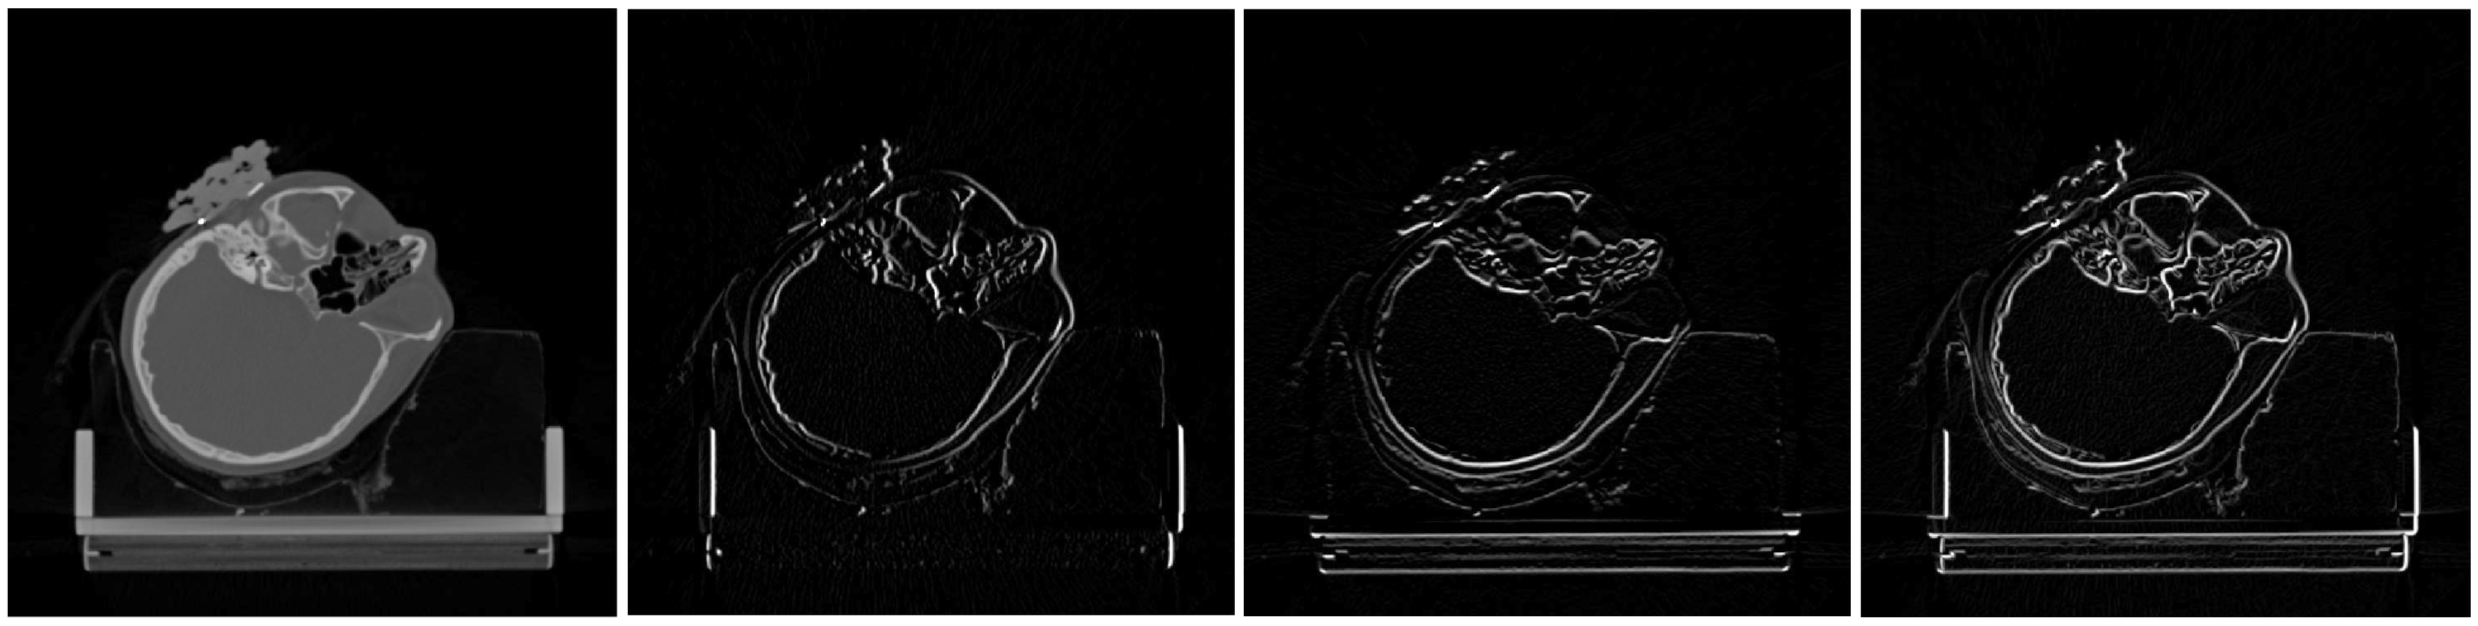
\includegraphics{beispiel_schaedel.png}
\end{figure}


    \hypertarget{sobel-operator-in-x-richtung}{%
\subsubsection*{Sobel-Operator in
x-Richtung}\label{sobel-operator-in-x-richtung}}

    \[\scriptstyle S_x =  \def\g{\color{lightgray}}\left(\begin{array}{rrr}0.25 & 0.0 & -0.25\\0.5 & 0.0 & -0.5\\0.25 & 0.0 & -0.25\end{array}\right)\]

    
    \[\scriptstyle \def\g{\color{lightgray}}\left(\begin{array}{rrrrrrrrrrrr}0\cdot 0.25 & 0\cdot 0.00 & 0\cdot -0.25 & \g{0} & \g{0} & \g{0} & \g{0} & \g{0} & \g{0} & \g{0} & \g{0} & \g{0}\\0\cdot 0.50 & 5\cdot 0.00 & 2\cdot -0.50 & \g{6} & \g{2} & \g{3} & \g{2} & \g{1} & \g{2} & \g{3} & \g{1} & \g{0}\\0\cdot 0.25 & 1\cdot 0.00 & 3\cdot -0.25 & \g{6} & \g{7} & \g{9} & \g{2} & \g{4} & \g{4} & \g{7} & \g{1} & \g{0}\\\g{0} & \g{1} & \g{5} & \g{8} & \g{8} & \g{10} & \g{17} & \g{21} & \g{19} & \g{9} & \g{4} & \g{0}\\\g{0} & \g{4} & \g{18} & \g{34} & \g{56} & \g{17} & \g{25} & \g{38} & \g{17} & \g{7} & \g{2} & \g{0}\\\g{0} & \g{1} & \g{14} & \g{22} & \g{43} & \g{68} & \g{91} & \g{62} & \g{23} & \g{16} & \g{7} & \g{0}\\\g{0} & \g{6} & \g{12} & \g{21} & \g{21} & \g{39} & \g{87} & \g{76} & \g{34} & \g{4} & \g{2} & \g{0}\\\g{0} & \g{9} & \g{24} & \g{54} & \g{73} & \g{88} & \g{95} & \g{69} & \g{16} & \g{12} & \g{5} & \g{0}\\\g{0} & \g{3} & \g{5} & \g{6} & \g{40} & \g{34} & \g{42} & \g{6} & \g{4} & \g{2} & \g{5} & \g{0}\\\g{0} & \g{4} & \g{9} & \g{16} & \g{14} & \g{32} & \g{51} & \g{13} & \g{6} & \g{6} & \g{2} & \g{0}\\\g{0} & \g{4} & \g{2} & \g{5} & \g{3} & \g{3} & \g{3} & \g{5} & \g{3} & \g{3} & \g{3} & \g{0}\\\g{0} & \g{0} & \g{0} & \g{0} & \g{0} & \g{0} & \g{0} & \g{0} & \g{0} & \g{0} & \g{0} & \g{0}\end{array}\right)=\left(\begin{array}{rrrrrrrrrrrr}-2 & \g{2} & \g{6} & \g{2} & \g{3} & \g{2} & \g{1} & \g{2} & \g{3} & \g{1}\\\g{1} & \g{3} & \g{6} & \g{7} & \g{9} & \g{2} & \g{4} & \g{4} & \g{7} & \g{1}\\\g{1} & \g{5} & \g{8} & \g{8} & \g{10} & \g{17} & \g{21} & \g{19} & \g{9} & \g{4}\\\g{4} & \g{18} & \g{34} & \g{56} & \g{17} & \g{25} & \g{38} & \g{17} & \g{7} & \g{2}\\\g{1} & \g{14} & \g{22} & \g{43} & \g{68} & \g{91} & \g{62} & \g{23} & \g{16} & \g{7}\\\g{6} & \g{12} & \g{21} & \g{21} & \g{39} & \g{87} & \g{76} & \g{34} & \g{4} & \g{2}\\\g{9} & \g{24} & \g{54} & \g{73} & \g{88} & \g{95} & \g{69} & \g{16} & \g{12} & \g{5}\\\g{3} & \g{5} & \g{6} & \g{40} & \g{34} & \g{42} & \g{6} & \g{4} & \g{2} & \g{5}\\\g{4} & \g{9} & \g{16} & \g{14} & \g{32} & \g{51} & \g{13} & \g{6} & \g{6} & \g{2}\\\g{4} & \g{2} & \g{5} & \g{3} & \g{3} & \g{3} & \g{5} & \g{3} & \g{3} & \g{3}\end{array}\right)\]

    
    \[\scriptstyle \def\g{\color{lightgray}}\left(\begin{array}{rrrrrrrrrrrr}\g{0} & 0\cdot 0.25 & 0\cdot 0.00 & 0\cdot -0.25 & \g{0} & \g{0} & \g{0} & \g{0} & \g{0} & \g{0} & \g{0} & \g{0}\\\g{0} & 5\cdot 0.50 & 2\cdot 0.00 & 6\cdot -0.50 & \g{2} & \g{3} & \g{2} & \g{1} & \g{2} & \g{3} & \g{1} & \g{0}\\\g{0} & 1\cdot 0.25 & 3\cdot 0.00 & 6\cdot -0.25 & \g{7} & \g{9} & \g{2} & \g{4} & \g{4} & \g{7} & \g{1} & \g{0}\\\g{0} & \g{1} & \g{5} & \g{8} & \g{8} & \g{10} & \g{17} & \g{21} & \g{19} & \g{9} & \g{4} & \g{0}\\\g{0} & \g{4} & \g{18} & \g{34} & \g{56} & \g{17} & \g{25} & \g{38} & \g{17} & \g{7} & \g{2} & \g{0}\\\g{0} & \g{1} & \g{14} & \g{22} & \g{43} & \g{68} & \g{91} & \g{62} & \g{23} & \g{16} & \g{7} & \g{0}\\\g{0} & \g{6} & \g{12} & \g{21} & \g{21} & \g{39} & \g{87} & \g{76} & \g{34} & \g{4} & \g{2} & \g{0}\\\g{0} & \g{9} & \g{24} & \g{54} & \g{73} & \g{88} & \g{95} & \g{69} & \g{16} & \g{12} & \g{5} & \g{0}\\\g{0} & \g{3} & \g{5} & \g{6} & \g{40} & \g{34} & \g{42} & \g{6} & \g{4} & \g{2} & \g{5} & \g{0}\\\g{0} & \g{4} & \g{9} & \g{16} & \g{14} & \g{32} & \g{51} & \g{13} & \g{6} & \g{6} & \g{2} & \g{0}\\\g{0} & \g{4} & \g{2} & \g{5} & \g{3} & \g{3} & \g{3} & \g{5} & \g{3} & \g{3} & \g{3} & \g{0}\\\g{0} & \g{0} & \g{0} & \g{0} & \g{0} & \g{0} & \g{0} & \g{0} & \g{0} & \g{0} & \g{0} & \g{0}\end{array}\right)=\left(\begin{array}{rrrrrrrrrrrr}\g{-2} & -2 & \g{6} & \g{2} & \g{3} & \g{2} & \g{1} & \g{2} & \g{3} & \g{1}\\\g{1} & \g{3} & \g{6} & \g{7} & \g{9} & \g{2} & \g{4} & \g{4} & \g{7} & \g{1}\\\g{1} & \g{5} & \g{8} & \g{8} & \g{10} & \g{17} & \g{21} & \g{19} & \g{9} & \g{4}\\\g{4} & \g{18} & \g{34} & \g{56} & \g{17} & \g{25} & \g{38} & \g{17} & \g{7} & \g{2}\\\g{1} & \g{14} & \g{22} & \g{43} & \g{68} & \g{91} & \g{62} & \g{23} & \g{16} & \g{7}\\\g{6} & \g{12} & \g{21} & \g{21} & \g{39} & \g{87} & \g{76} & \g{34} & \g{4} & \g{2}\\\g{9} & \g{24} & \g{54} & \g{73} & \g{88} & \g{95} & \g{69} & \g{16} & \g{12} & \g{5}\\\g{3} & \g{5} & \g{6} & \g{40} & \g{34} & \g{42} & \g{6} & \g{4} & \g{2} & \g{5}\\\g{4} & \g{9} & \g{16} & \g{14} & \g{32} & \g{51} & \g{13} & \g{6} & \g{6} & \g{2}\\\g{4} & \g{2} & \g{5} & \g{3} & \g{3} & \g{3} & \g{5} & \g{3} & \g{3} & \g{3}\end{array}\right)\]

    
    \[\scriptstyle \def\g{\color{lightgray}}\left(\begin{array}{rrrrrrrrrrrr}\g{0} & \g{0} & 0\cdot 0.25 & 0\cdot 0.00 & 0\cdot -0.25 & \g{0} & \g{0} & \g{0} & \g{0} & \g{0} & \g{0} & \g{0}\\\g{0} & \g{5} & 2\cdot 0.50 & 6\cdot 0.00 & 2\cdot -0.50 & \g{3} & \g{2} & \g{1} & \g{2} & \g{3} & \g{1} & \g{0}\\\g{0} & \g{1} & 3\cdot 0.25 & 6\cdot 0.00 & 7\cdot -0.25 & \g{9} & \g{2} & \g{4} & \g{4} & \g{7} & \g{1} & \g{0}\\\g{0} & \g{1} & \g{5} & \g{8} & \g{8} & \g{10} & \g{17} & \g{21} & \g{19} & \g{9} & \g{4} & \g{0}\\\g{0} & \g{4} & \g{18} & \g{34} & \g{56} & \g{17} & \g{25} & \g{38} & \g{17} & \g{7} & \g{2} & \g{0}\\\g{0} & \g{1} & \g{14} & \g{22} & \g{43} & \g{68} & \g{91} & \g{62} & \g{23} & \g{16} & \g{7} & \g{0}\\\g{0} & \g{6} & \g{12} & \g{21} & \g{21} & \g{39} & \g{87} & \g{76} & \g{34} & \g{4} & \g{2} & \g{0}\\\g{0} & \g{9} & \g{24} & \g{54} & \g{73} & \g{88} & \g{95} & \g{69} & \g{16} & \g{12} & \g{5} & \g{0}\\\g{0} & \g{3} & \g{5} & \g{6} & \g{40} & \g{34} & \g{42} & \g{6} & \g{4} & \g{2} & \g{5} & \g{0}\\\g{0} & \g{4} & \g{9} & \g{16} & \g{14} & \g{32} & \g{51} & \g{13} & \g{6} & \g{6} & \g{2} & \g{0}\\\g{0} & \g{4} & \g{2} & \g{5} & \g{3} & \g{3} & \g{3} & \g{5} & \g{3} & \g{3} & \g{3} & \g{0}\\\g{0} & \g{0} & \g{0} & \g{0} & \g{0} & \g{0} & \g{0} & \g{0} & \g{0} & \g{0} & \g{0} & \g{0}\end{array}\right)=\left(\begin{array}{rrrrrrrrrrrr}\g{-2} & \g{-2} & -1 & \g{2} & \g{3} & \g{2} & \g{1} & \g{2} & \g{3} & \g{1}\\\g{1} & \g{3} & \g{6} & \g{7} & \g{9} & \g{2} & \g{4} & \g{4} & \g{7} & \g{1}\\\g{1} & \g{5} & \g{8} & \g{8} & \g{10} & \g{17} & \g{21} & \g{19} & \g{9} & \g{4}\\\g{4} & \g{18} & \g{34} & \g{56} & \g{17} & \g{25} & \g{38} & \g{17} & \g{7} & \g{2}\\\g{1} & \g{14} & \g{22} & \g{43} & \g{68} & \g{91} & \g{62} & \g{23} & \g{16} & \g{7}\\\g{6} & \g{12} & \g{21} & \g{21} & \g{39} & \g{87} & \g{76} & \g{34} & \g{4} & \g{2}\\\g{9} & \g{24} & \g{54} & \g{73} & \g{88} & \g{95} & \g{69} & \g{16} & \g{12} & \g{5}\\\g{3} & \g{5} & \g{6} & \g{40} & \g{34} & \g{42} & \g{6} & \g{4} & \g{2} & \g{5}\\\g{4} & \g{9} & \g{16} & \g{14} & \g{32} & \g{51} & \g{13} & \g{6} & \g{6} & \g{2}\\\g{4} & \g{2} & \g{5} & \g{3} & \g{3} & \g{3} & \g{5} & \g{3} & \g{3} & \g{3}\end{array}\right)\]

    
    \[\scriptstyle x =  \def\g{\color{lightgray}}\left(\begin{array}{rrrrrrrrrr}-2 & -2 & -1 & 1 & 1 & 2 & 0 & -2 & 1 & 3\\-3 & -4 & -3 & -1 & 0 & 0 & -2 & 1 & 6 & 6\\-8 & -12 & -12 & 2 & 4 & -10 & 0 & 13 & 12 & 8\\-14 & -22 & -27 & -4 & 1 & -12 & 20 & 30 & 15 & 10\\-14 & -22 & -26 & -23 & -33 & -12 & 49 & 49 & 20 & 11\\-16 & -24 & -24 & -29 & -50 & -12 & 63 & 62 & 23 & 9\\-16 & -27 & -36 & -28 & -28 & 7 & 62 & 48 & 13 & 8\\-11 & -16 & -31 & -26 & -16 & 24 & 50 & 18 & 3 & 6\\-6 & -7 & -12 & -14 & -19 & 16 & 32 & 5 & 2 & 4\\-3 & -4 & -2 & -3 & -9 & 4 & 11 & 3 & 1 & 3\end{array}\right)\]

    
    \[\scriptstyle x\_spread =  \def\g{\color{lightgray}}\left(\begin{array}{rrrrrrrrrr}109 & 109 & 111 & 114 & 116 & 118 & 112 & 109 & 116 & 120\\106 & 103 & 107 & 110 & 113 & 113 & 109 & 115 & 125 & 127\\95 & 85 & 86 & 118 & 123 & 92 & 114 & 142 & 140 & 131\\82 & 64 & 52 & 105 & 116 & 87 & 159 & 180 & 147 & 135\\80 & 64 & 54 & 61 & 40 & 87 & 223 & 222 & 157 & 137\\78 & 59 & 59 & 48 & 0 & 85 & 254 & 251 & 164 & 133\\76 & 52 & 33 & 49 & 50 & 129 & 252 & 219 & 142 & 130\\89 & 78 & 44 & 54 & 78 & 165 & 224 & 153 & 120 & 125\\99 & 97 & 87 & 80 & 70 & 148 & 184 & 124 & 117 & 122\\106 & 105 & 109 & 106 & 92 & 121 & 138 & 119 & 115 & 119\end{array}\right)\]


\newpage    
    \hypertarget{sobel-operator-in-y-richtung}{%
\subsubsection*{Sobel-Operator in
y-Richtung}\label{sobel-operator-in-y-richtung}}

    \[\scriptstyle S_y =  \def\g{\color{lightgray}}\left(\begin{array}{rrr}0.25 & 0.5 & 0.25\\0.0 & 0.0 & 0.0\\-0.25 & -0.5 & -0.25\end{array}\right)\]

    
    \[\scriptstyle \def\g{\color{lightgray}}\left(\begin{array}{rrrrrrrrrrrr}0\cdot 0.25 & 0\cdot 0.50 & 0\cdot 0.25 & \g{0} & \g{0} & \g{0} & \g{0} & \g{0} & \g{0} & \g{0} & \g{0} & \g{0}\\0\cdot 0.00 & 5\cdot 0.00 & 2\cdot 0.00 & \g{6} & \g{2} & \g{3} & \g{2} & \g{1} & \g{2} & \g{3} & \g{1} & \g{0}\\0\cdot -0.25 & 1\cdot -0.50 & 3\cdot -0.25 & \g{6} & \g{7} & \g{9} & \g{2} & \g{4} & \g{4} & \g{7} & \g{1} & \g{0}\\\g{0} & \g{1} & \g{5} & \g{8} & \g{8} & \g{10} & \g{17} & \g{21} & \g{19} & \g{9} & \g{4} & \g{0}\\\g{0} & \g{4} & \g{18} & \g{34} & \g{56} & \g{17} & \g{25} & \g{38} & \g{17} & \g{7} & \g{2} & \g{0}\\\g{0} & \g{1} & \g{14} & \g{22} & \g{43} & \g{68} & \g{91} & \g{62} & \g{23} & \g{16} & \g{7} & \g{0}\\\g{0} & \g{6} & \g{12} & \g{21} & \g{21} & \g{39} & \g{87} & \g{76} & \g{34} & \g{4} & \g{2} & \g{0}\\\g{0} & \g{9} & \g{24} & \g{54} & \g{73} & \g{88} & \g{95} & \g{69} & \g{16} & \g{12} & \g{5} & \g{0}\\\g{0} & \g{3} & \g{5} & \g{6} & \g{40} & \g{34} & \g{42} & \g{6} & \g{4} & \g{2} & \g{5} & \g{0}\\\g{0} & \g{4} & \g{9} & \g{16} & \g{14} & \g{32} & \g{51} & \g{13} & \g{6} & \g{6} & \g{2} & \g{0}\\\g{0} & \g{4} & \g{2} & \g{5} & \g{3} & \g{3} & \g{3} & \g{5} & \g{3} & \g{3} & \g{3} & \g{0}\\\g{0} & \g{0} & \g{0} & \g{0} & \g{0} & \g{0} & \g{0} & \g{0} & \g{0} & \g{0} & \g{0} & \g{0}\end{array}\right)=\left(\begin{array}{rrrrrrrrrrrr}-1 & \g{2} & \g{6} & \g{2} & \g{3} & \g{2} & \g{1} & \g{2} & \g{3} & \g{1}\\\g{1} & \g{3} & \g{6} & \g{7} & \g{9} & \g{2} & \g{4} & \g{4} & \g{7} & \g{1}\\\g{1} & \g{5} & \g{8} & \g{8} & \g{10} & \g{17} & \g{21} & \g{19} & \g{9} & \g{4}\\\g{4} & \g{18} & \g{34} & \g{56} & \g{17} & \g{25} & \g{38} & \g{17} & \g{7} & \g{2}\\\g{1} & \g{14} & \g{22} & \g{43} & \g{68} & \g{91} & \g{62} & \g{23} & \g{16} & \g{7}\\\g{6} & \g{12} & \g{21} & \g{21} & \g{39} & \g{87} & \g{76} & \g{34} & \g{4} & \g{2}\\\g{9} & \g{24} & \g{54} & \g{73} & \g{88} & \g{95} & \g{69} & \g{16} & \g{12} & \g{5}\\\g{3} & \g{5} & \g{6} & \g{40} & \g{34} & \g{42} & \g{6} & \g{4} & \g{2} & \g{5}\\\g{4} & \g{9} & \g{16} & \g{14} & \g{32} & \g{51} & \g{13} & \g{6} & \g{6} & \g{2}\\\g{4} & \g{2} & \g{5} & \g{3} & \g{3} & \g{3} & \g{5} & \g{3} & \g{3} & \g{3}\end{array}\right)\]

    
    \[\scriptstyle \def\g{\color{lightgray}}\left(\begin{array}{rrrrrrrrrrrr}\g{0} & 0\cdot 0.25 & 0\cdot 0.50 & 0\cdot 0.25 & \g{0} & \g{0} & \g{0} & \g{0} & \g{0} & \g{0} & \g{0} & \g{0}\\\g{0} & 5\cdot 0.00 & 2\cdot 0.00 & 6\cdot 0.00 & \g{2} & \g{3} & \g{2} & \g{1} & \g{2} & \g{3} & \g{1} & \g{0}\\\g{0} & 1\cdot -0.25 & 3\cdot -0.50 & 6\cdot -0.25 & \g{7} & \g{9} & \g{2} & \g{4} & \g{4} & \g{7} & \g{1} & \g{0}\\\g{0} & \g{1} & \g{5} & \g{8} & \g{8} & \g{10} & \g{17} & \g{21} & \g{19} & \g{9} & \g{4} & \g{0}\\\g{0} & \g{4} & \g{18} & \g{34} & \g{56} & \g{17} & \g{25} & \g{38} & \g{17} & \g{7} & \g{2} & \g{0}\\\g{0} & \g{1} & \g{14} & \g{22} & \g{43} & \g{68} & \g{91} & \g{62} & \g{23} & \g{16} & \g{7} & \g{0}\\\g{0} & \g{6} & \g{12} & \g{21} & \g{21} & \g{39} & \g{87} & \g{76} & \g{34} & \g{4} & \g{2} & \g{0}\\\g{0} & \g{9} & \g{24} & \g{54} & \g{73} & \g{88} & \g{95} & \g{69} & \g{16} & \g{12} & \g{5} & \g{0}\\\g{0} & \g{3} & \g{5} & \g{6} & \g{40} & \g{34} & \g{42} & \g{6} & \g{4} & \g{2} & \g{5} & \g{0}\\\g{0} & \g{4} & \g{9} & \g{16} & \g{14} & \g{32} & \g{51} & \g{13} & \g{6} & \g{6} & \g{2} & \g{0}\\\g{0} & \g{4} & \g{2} & \g{5} & \g{3} & \g{3} & \g{3} & \g{5} & \g{3} & \g{3} & \g{3} & \g{0}\\\g{0} & \g{0} & \g{0} & \g{0} & \g{0} & \g{0} & \g{0} & \g{0} & \g{0} & \g{0} & \g{0} & \g{0}\end{array}\right)=\left(\begin{array}{rrrrrrrrrrrr}\g{-1} & -3 & \g{6} & \g{2} & \g{3} & \g{2} & \g{1} & \g{2} & \g{3} & \g{1}\\\g{1} & \g{3} & \g{6} & \g{7} & \g{9} & \g{2} & \g{4} & \g{4} & \g{7} & \g{1}\\\g{1} & \g{5} & \g{8} & \g{8} & \g{10} & \g{17} & \g{21} & \g{19} & \g{9} & \g{4}\\\g{4} & \g{18} & \g{34} & \g{56} & \g{17} & \g{25} & \g{38} & \g{17} & \g{7} & \g{2}\\\g{1} & \g{14} & \g{22} & \g{43} & \g{68} & \g{91} & \g{62} & \g{23} & \g{16} & \g{7}\\\g{6} & \g{12} & \g{21} & \g{21} & \g{39} & \g{87} & \g{76} & \g{34} & \g{4} & \g{2}\\\g{9} & \g{24} & \g{54} & \g{73} & \g{88} & \g{95} & \g{69} & \g{16} & \g{12} & \g{5}\\\g{3} & \g{5} & \g{6} & \g{40} & \g{34} & \g{42} & \g{6} & \g{4} & \g{2} & \g{5}\\\g{4} & \g{9} & \g{16} & \g{14} & \g{32} & \g{51} & \g{13} & \g{6} & \g{6} & \g{2}\\\g{4} & \g{2} & \g{5} & \g{3} & \g{3} & \g{3} & \g{5} & \g{3} & \g{3} & \g{3}\end{array}\right)\]

    
    \[\scriptstyle \def\g{\color{lightgray}}\left(\begin{array}{rrrrrrrrrrrr}\g{0} & \g{0} & 0\cdot 0.25 & 0\cdot 0.50 & 0\cdot 0.25 & \g{0} & \g{0} & \g{0} & \g{0} & \g{0} & \g{0} & \g{0}\\\g{0} & \g{5} & 2\cdot 0.00 & 6\cdot 0.00 & 2\cdot 0.00 & \g{3} & \g{2} & \g{1} & \g{2} & \g{3} & \g{1} & \g{0}\\\g{0} & \g{1} & 3\cdot -0.25 & 6\cdot -0.50 & 7\cdot -0.25 & \g{9} & \g{2} & \g{4} & \g{4} & \g{7} & \g{1} & \g{0}\\\g{0} & \g{1} & \g{5} & \g{8} & \g{8} & \g{10} & \g{17} & \g{21} & \g{19} & \g{9} & \g{4} & \g{0}\\\g{0} & \g{4} & \g{18} & \g{34} & \g{56} & \g{17} & \g{25} & \g{38} & \g{17} & \g{7} & \g{2} & \g{0}\\\g{0} & \g{1} & \g{14} & \g{22} & \g{43} & \g{68} & \g{91} & \g{62} & \g{23} & \g{16} & \g{7} & \g{0}\\\g{0} & \g{6} & \g{12} & \g{21} & \g{21} & \g{39} & \g{87} & \g{76} & \g{34} & \g{4} & \g{2} & \g{0}\\\g{0} & \g{9} & \g{24} & \g{54} & \g{73} & \g{88} & \g{95} & \g{69} & \g{16} & \g{12} & \g{5} & \g{0}\\\g{0} & \g{3} & \g{5} & \g{6} & \g{40} & \g{34} & \g{42} & \g{6} & \g{4} & \g{2} & \g{5} & \g{0}\\\g{0} & \g{4} & \g{9} & \g{16} & \g{14} & \g{32} & \g{51} & \g{13} & \g{6} & \g{6} & \g{2} & \g{0}\\\g{0} & \g{4} & \g{2} & \g{5} & \g{3} & \g{3} & \g{3} & \g{5} & \g{3} & \g{3} & \g{3} & \g{0}\\\g{0} & \g{0} & \g{0} & \g{0} & \g{0} & \g{0} & \g{0} & \g{0} & \g{0} & \g{0} & \g{0} & \g{0}\end{array}\right)=\left(\begin{array}{rrrrrrrrrrrr}\g{-1} & \g{-3} & -6 & \g{2} & \g{3} & \g{2} & \g{1} & \g{2} & \g{3} & \g{1}\\\g{1} & \g{3} & \g{6} & \g{7} & \g{9} & \g{2} & \g{4} & \g{4} & \g{7} & \g{1}\\\g{1} & \g{5} & \g{8} & \g{8} & \g{10} & \g{17} & \g{21} & \g{19} & \g{9} & \g{4}\\\g{4} & \g{18} & \g{34} & \g{56} & \g{17} & \g{25} & \g{38} & \g{17} & \g{7} & \g{2}\\\g{1} & \g{14} & \g{22} & \g{43} & \g{68} & \g{91} & \g{62} & \g{23} & \g{16} & \g{7}\\\g{6} & \g{12} & \g{21} & \g{21} & \g{39} & \g{87} & \g{76} & \g{34} & \g{4} & \g{2}\\\g{9} & \g{24} & \g{54} & \g{73} & \g{88} & \g{95} & \g{69} & \g{16} & \g{12} & \g{5}\\\g{3} & \g{5} & \g{6} & \g{40} & \g{34} & \g{42} & \g{6} & \g{4} & \g{2} & \g{5}\\\g{4} & \g{9} & \g{16} & \g{14} & \g{32} & \g{51} & \g{13} & \g{6} & \g{6} & \g{2}\\\g{4} & \g{2} & \g{5} & \g{3} & \g{3} & \g{3} & \g{5} & \g{3} & \g{3} & \g{3}\end{array}\right)\]

    
    \[\scriptstyle y =  \def\g{\color{lightgray}}\left(\begin{array}{rrrrrrrrrr}-1 & -3 & -6 & -7 & -7 & -4 & -4 & -5 & -5 & -2\\1 & -1 & -3 & -5 & -9 & -14 & -18 & -15 & -8 & -3\\-5 & -15 & -30 & -34 & -22 & -22 & -26 & -15 & -4 & 0\\-2 & -8 & -18 & -36 & -56 & -62 & -40 & -14 & -5 & -3\\0 & 6 & 17 & 15 & -18 & -46 & -39 & -17 & -3 & 1\\-6 & -15 & -26 & -28 & -18 & -9 & -3 & 3 & 4 & 2\\3 & 8 & 4 & -4 & 9 & 41 & 54 & 33 & 8 & -1\\6 & 18 & 38 & 53 & 54 & 50 & 42 & 20 & 6 & 3\\0 & 2 & 10 & 26 & 34 & 28 & 10 & 0 & 0 & 1\\4 & 10 & 14 & 19 & 32 & 37 & 21 & 8 & 5 & 2\end{array}\right)\]

    
    \[\scriptstyle y\_spread =  \def\g{\color{lightgray}}\left(\begin{array}{rrrrrrrrrr}133 & 129 & 124 & 120 & 121 & 126 & 128 & 125 & 125 & 131\\139 & 134 & 129 & 124 & 117 & 104 & 96 & 103 & 118 & 129\\124 & 102 & 70 & 62 & 87 & 87 & 79 & 103 & 128 & 135\\131 & 118 & 96 & 58 & 12 & 0 & 48 & 105 & 124 & 129\\137 & 148 & 173 & 169 & 97 & 35 & 51 & 98 & 130 & 137\\122 & 103 & 79 & 74 & 95 & 117 & 130 & 142 & 145 & 140\\143 & 153 & 146 & 126 & 156 & 227 & 254 & 208 & 153 & 134\\150 & 176 & 218 & 252 & 254 & 246 & 227 & 181 & 150 & 142\\136 & 139 & 159 & 194 & 212 & 196 & 159 & 137 & 136 & 137\\145 & 157 & 166 & 178 & 207 & 217 & 181 & 153 & 147 & 141\end{array}\right)\]

\newpage
    
    \hypertarget{berechnung-der-kanten-sobel-operator-max}{%
\section*{3) Berechnung der Kanten
(Sobel-Operator-Max)}\label{berechnung-der-kanten-sobel-operator-max}}


    \[\scriptstyle g =  \def\g{\color{lightgray}}\left(\begin{array}{rrrrrrrrrr}2 & 3 & 6 & 7 & 7 & 4 & 4 & 5 & 5 & 3\\3 & 4 & 3 & 5 & 9 & 14 & 18 & 15 & 8 & 6\\8 & 15 & 30 & 34 & 22 & 22 & 26 & 15 & 12 & 8\\14 & 22 & 27 & 36 & 56 & 62 & 40 & 30 & 15 & 10\\14 & 22 & 26 & 23 & 33 & 46 & 49 & 49 & 20 & 11\\16 & 24 & 26 & 29 & 50 & 12 & 63 & 62 & 23 & 9\\16 & 27 & 36 & 28 & 28 & 41 & 62 & 48 & 13 & 8\\11 & 18 & 38 & 53 & 54 & 50 & 50 & 20 & 6 & 6\\6 & 7 & 12 & 26 & 34 & 28 & 32 & 5 & 2 & 4\\4 & 10 & 14 & 19 & 32 & 37 & 21 & 8 & 5 & 3\end{array}\right)\]

    
    \[\scriptstyle g\_spread =  \def\g{\color{lightgray}}\left(\begin{array}{rrrrrrrrrr}0 & 6 & 15 & 23 & 21 & 10 & 7 & 12 & 12 & 6\\6 & 11 & 6 & 14 & 29 & 52 & 67 & 55 & 26 & 20\\25 & 56 & 117 & 131 & 84 & 84 & 100 & 55 & 42 & 26\\50 & 84 & 104 & 139 & 225 & 248 & 158 & 117 & 56 & 33\\53 & 83 & 101 & 89 & 128 & 183 & 196 & 194 & 74 & 37\\57 & 92 & 100 & 113 & 201 & 43 & 254 & 248 & 87 & 30\\60 & 104 & 139 & 110 & 108 & 163 & 250 & 189 & 47 & 24\\37 & 68 & 148 & 212 & 215 & 199 & 199 & 77 & 19 & 15\\19 & 22 & 40 & 102 & 135 & 106 & 125 & 13 & 0 & 10\\10 & 32 & 50 & 71 & 126 & 145 & 78 & 25 & 13 & 5\end{array}\right)\]

    \begin{center}
    \adjustimage{max size={0.9\linewidth}{0.9\paperheight}}{output_19_3.png}
    \end{center}
    { \hspace*{\fill} \\}
    
    \hypertarget{darstellungen-der-einzelnen-schritte}{%
\section*{4) Darstellungen der einzelnen
Schritte}\label{darstellungen-der-einzelnen-schritte}}

    \begin{center}
    \adjustimage{max size={0.9\linewidth}{0.9\paperheight}}{output_21_0.png}
    \end{center}
    { \hspace*{\fill} \\}
    

    % Add a bibliography block to the postdoc
    
    
    
    \end{document}
